\documentclass[tikz,border=5pt]{standalone}
\usepackage{luatexja}
\usepackage[hiragino-pron]{luatexja-preset}
\usepackage{amsmath,amssymb,bm}
\usetikzlibrary{arrows.meta}

\begin{document}
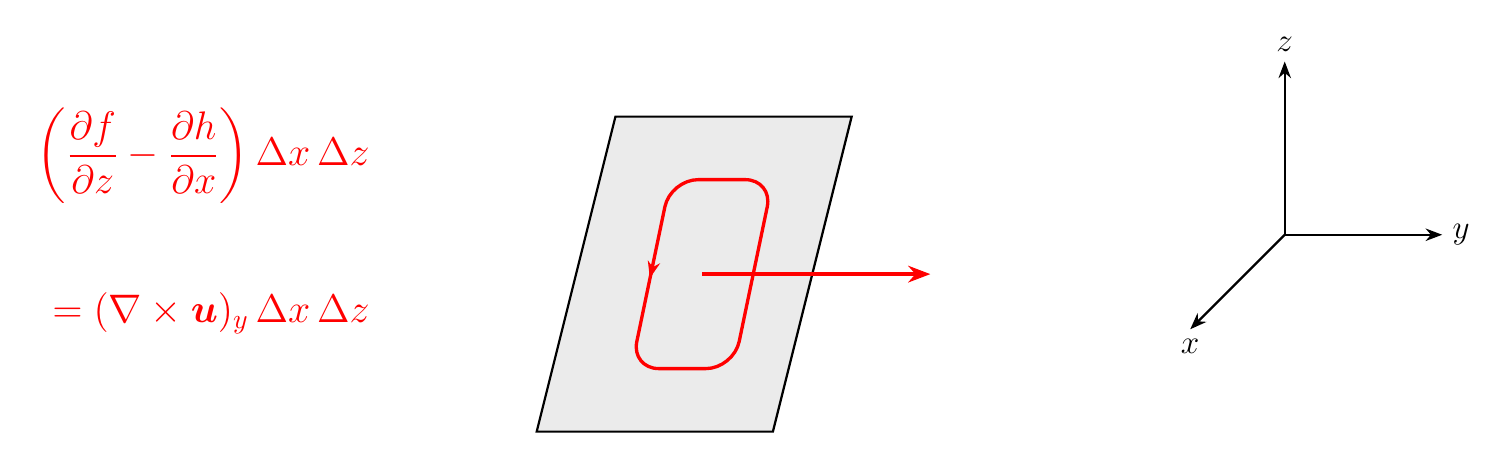
\begin{tikzpicture}[every node/.style={font=\large}]

  %% Left: formula
  \node[red, font=\Large, anchor=east] at (0,1.5) {$\left(\dfrac{\partial f}{\partial z} - \dfrac{\partial h}{\partial x}\right) \Delta x\, \Delta z$};
  \node[red, font=\Large, anchor=east] at (0,-0.5) {$= (\nabla \times \boldsymbol{u})_y\, \Delta x\, \Delta z$};

  %% Center: xz-plane with circulation and y-component arrow
  \begin{scope}[xshift=4cm]
    % Parallelogram for xz-plane (perspective view, vertical plane)
    \fill[black!8] (-2,-2) -- (1,-2) -- (2,2) -- (-1,2) -- cycle;
    \draw[thick] (-2,-2) -- (1,-2) -- (2,2) -- (-1,2) -- cycle;

    % Circulation arrow (red, clockwise)
    \draw[very thick, red, rounded corners=10pt]
      (-0.8,-1.2) -- (0.5,-1.2) -- (1.0,1.2) -- (-0.3,1.2) -- cycle;
    % Arrowhead on left edge (midpoint going downward)
    \draw[-{Stealth[length=6pt]}, very thick, red] (-0.55,0.0) -- (-0.5625,-0.05);

    % y-component arrow (red, pointing right / out of plane)
    \draw[-{Stealth[length=8pt]}, ultra thick, red] (0.1,0) -- (3.0,0);
  \end{scope}

  %% Right: xyz axes
  \begin{scope}[xshift=11.5cm, yshift=0.5cm]
    \draw[-{Stealth[length=6pt]}, thick] (0,0) -- (0,2.2) node[above] {$z$};
    \draw[-{Stealth[length=6pt]}, thick] (0,0) -- (2,0) node[right] {$y$};
    \draw[-{Stealth[length=6pt]}, thick] (0,0) -- (-1.2,-1.2) node[below] {$x$};
  \end{scope}

\end{tikzpicture}
\end{document}
